\documentclass[12pt, a4paper]{report}
\usepackage{graphicx, array, amsthm, amssymb, amsmath, algorithm, algpseudocode, float, xcolor, thmtools, thmbox, exercise}
\usepackage[english]{babel}

\makeatletter
\renewcommand\thmbox@headstyle[2]{\bfseries #1}
\makeatother
\newtheorem[style=M,bodystyle=\normalfont]{theorem}{Theorem}
\newtheorem[style=M,bodystyle=\normalfont]{corollary}{Corollary}
\newtheorem[style=M,bodystyle=\normalfont]{lemma}{Lemma}
\newtheorem[style=M,bodystyle=\normalfont]{definition}{Definition}


\title{Data Bases II \\ \textit{Exercises}}
\author{Christian Rossi}
\date{Academic Year 2023-2024}

\begin{document}

\maketitle

\newpage

\begin{abstract}
    The course aims to prepare software designers on the effective development of database applications. 
    
    First, the course presents the fundamental features of current database architectures, with a specific emphasis on the concept of transaction and its realization in centralized 
    and distributed systems. 
    
    Then, the course illustrates the main directions in the evolution of database systems, presenting approaches that go beyond the relational model, like active databases, object 
    systems and XML data management solutions.
\end{abstract}

\newpage

\tableofcontents

\newpage

\chapter{Exercise session I}
    \begin{Exercise}[label=1]
        Can the following schedules produce anomalies? $c_i$ and $a_i$ indicate the transactional decision (commit/abort). 
        \begin{enumerate}
            \item $r_1(x) w_1(x) r_2(x) w_2(y)\:a_1\:c_2$
            \item $r_1(x) w_1(x) r_2(y) w_2(y)\:a_1\:c_2$
            \item $r_1(x) r_2(x) r_2(y) w_2(y) r_1(z)\:a_1\:c_2$
            \item $r_1(x) r_2(x) w_2(x) w_1(x)\:c_1\:c_2$
            \item $r_1(x) r_2(x) w_2(x) r_1(y)\:c_1\:c_2$
            \item $r_1(x) w_1(x) r_2(x) w_2(x)\:c_1\:c_2$
        \end{enumerate}
    \end{Exercise}
    \begin{Answer}[ref=1]
        \begin{enumerate}
            \item We have a serial execution, but with the abort of the first transaction. Since the second transaction reads the modified value of $x$ before the abort, we have a
                dirty read. 
            \item We have a serial execution and the two transactions require different resources, so there are no anomalies.
            \item There are no anomalies because the last operation of the first transaction works on a different resource. 
            \item Both transactions first reads in sequence the resource $x$ and then updates it without considering the updated value, so we have a lost update. 
            \item There are no anomalies because the last operation of the first transaction works on a different resource. 
            \item We have a serial execution, so the schedule is correct. 
        \end{enumerate}
    \end{Answer}

    \newpage
    
    \begin{Exercise}[label=2]
        The following schedule may produce 2 anomalies: a lost update and a phantom update. Identify them. 
        \[r_1(x) r_2(x) r_3(x) w_1(x) r_4(y) w_2(x) r_4(x) w_4(y) r_3(y)w_4(x) r_5(y) w_6(y) w_5(y) w_7(y)\]
    \end{Exercise}
    \begin{Answer}[ref=2]
        We can write the schedule in the following way:
    \begin{table}[H]
        \centering
        \resizebox{\textwidth}{!}{%
        \begin{tabular}{cccccccccccccc}
        $r_1(x)$           &           &                    & $w_1(x)$           & \textbf{} & \textbf{} & \textbf{} & \textbf{} & \textbf{} & \textbf{} & \textbf{} & \textbf{} & \textbf{} & \textbf{} \\
                        & $r_2(x)$  & \textit{\textbf{}} & \textit{\textbf{}} & \textbf{} & $w_2(x)$  & \textbf{} & \textbf{} & \textbf{} & \textbf{} & \textbf{} & \textbf{} & \textbf{} & \textbf{} \\
        \textit{\textbf{}} & \textbf{} & $r_3(x)$           & \textbf{}          & \textbf{} & \textbf{} & \textbf{} & \textbf{} & $r_3(y)$  & \textbf{} & \textbf{} & \textbf{} & \textbf{} & \textbf{} \\
        \textit{\textbf{}} & \textbf{} & \textbf{}          &                    & $r_4(y)$  & \textbf{} & $r_4(x)$  & $w_4(y)$  & \textbf{} & $w_4(x)$  & \textbf{} & \textbf{} & \textbf{} & \textbf{} \\
        \textit{\textbf{}} & \textbf{} & \textbf{}          & \textbf{}          & \textbf{} & \textbf{} & \textbf{} & \textbf{} & \textbf{} & \textbf{} & $r_5(y)$  & \textbf{} & $w_5(y)$  & \textbf{} \\
        \textbf{}          & \textbf{} & \textbf{}          & \textbf{}          & \textbf{} & \textbf{} & \textbf{} & \textbf{} & \textbf{} & \textbf{} & \textbf{} & $w_6(y)$  & \textbf{} & \textbf{} \\
        \textbf{}          & \textbf{} & \textbf{}          & \textbf{}          & \textbf{} & \textbf{} & \textbf{} & \textbf{} & \textbf{} & \textbf{} & \textbf{} & \textbf{} & \textbf{} & $w_7(y)$ 
        \end{tabular}%
        }
    \end{table}
        And we can see that there is a lost update with transactions $T_1$ and $T_2$ and a phantom update with $T_3$ and $T_4$. 
    \end{Answer}

    \newpage
    
    \begin{Exercise}[label=3]
        Classify the following schedule with respect to $CRT$ and $VRT$ classes: 
        \[r_1(x) r_2(y) w_3(y) r_5(x) w_5(u) w_3(s)w_2(u) w_3(x) w_1(u) r_4(y) w_5(z) r_5(z)\]
    \end{Exercise}
    \begin{Answer}[ref=3]
        Since CSR contains VSR we check with the conflict graph. To do so we first divide the schedule based on the resources: 
        \begin{itemize}
            \item $x: r_1 \: r_5 \:w_3$
            \item $y: r_2 \: w_3 \:r_4$
            \item $z: w_5 \: r_5$
            \item $s: w_3$
            \item $u: w_5 \: w_2 \:w_1$
        \end{itemize}
        The nodes are $\{1,2,3,4,5\}$ and the arcs are found with the write-write or write-read relations found in the previous groups. So we have the following graph:
        \begin{figure}[H]
            \centering
            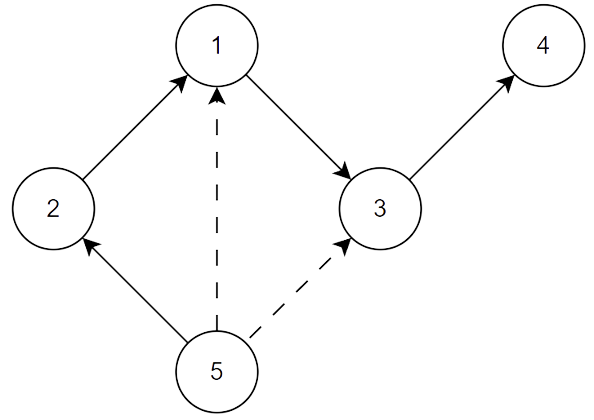
\includegraphics[width=0.5\linewidth]{images/conflictgraph.png}
        \end{figure}
        Some arcs can be omitted if the nodes are connected in another way (in this case we can remove arcs $\{\{5,1\},\{5,3\}\}$). 

        There are no cycles: the schedule is CSR (and also VSR). 
    \end{Answer}

    \newpage
    
    \begin{Exercise}[label=4]
        Classify the following schedule with respect to $CRT$ and $VRT$ classes: 
        \[r_2(u) w_2(s) r_1(x) r_2(y) w_3(y) r_5(x) w_5(u) w_3(s)w_2(u) w_3(x) w_1(u) r_4(y) w_5(z) r_5(z)\]
    \end{Exercise}
    \begin{Answer}[ref=4]
        Since CSR contains VSR we check with the conflict graph. To do so we first divide the schedule based on the resources: 
        \begin{itemize}
            \item $x: r_1 \: r_5 \:w_3$
            \item $y: r_2 \: w_3 \:r_4$
            \item $z: w_5 \: r_5$
            \item $s: w_2 \: w_3$
            \item $u: r_2 \: w_5 \: w_2 \:w_1$
        \end{itemize}
        The nodes are $\{1,2,3,4,5\}$ and the arcs are found with the write-write or write-read relations found in the previous groups. So we have the following graph:
        \begin{figure}[H]
            \centering
            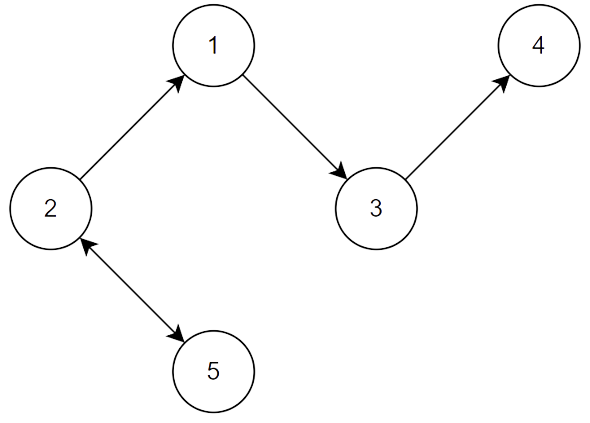
\includegraphics[width=0.5\linewidth]{images/conflictgraph1.png}
        \end{figure}
        It is possible to see that there is a cycle between two and five. The definition of VSR states that we need to have the same reads-from relations and final writes. So, we try to find a view-equivalent 
        schedule that is also CSR. One possible solution is simply to swap the two writes on the resource $u$ and that is sufficient to eliminate the cycle. So, the schedule: 
        \[r_2(u) w_2(s) r_1(x) r_2(y) w_3(y) r_5(x) w_5(u) w_2(u) w_3(s) w_3(x) w_1(u) r_4(y) w_5(z) r_5(z)\]
        is CSR and also VSR. 
    \end{Answer}

    \newpage
    
    \begin{Exercise}[label=5]
        Classify the following schedule with respect to $CRT$ and $VRT$ classes: 
        \[r_1(x) r_2(y) w_3(y) r_5(x) w_5(u) w_3(s)w_2(u) w_3(x) w_1(u) r_4(y) w_5(z) r_5(z) r_2(u) w_2(s)\]
    \end{Exercise}
    \begin{Answer}[ref=5]
        Since CSR contains VSR we check with the conflict graph. To do so we first divide the schedule based on the resources: 
        \begin{itemize}
            \item $x: r_1 \: r_5 \: w_3$
            \item $y: r_2 \: w_3 \: r_4$
            \item $z: w_5 \: r_5$
            \item $s: w_3 \: w_2$
            \item $u: w_5 \: w_2 \: w_1 \: r_2$
        \end{itemize}
        The nodes are $\{1,2,3,4,5\}$ and the arcs are found with the write-write or write-read relations found in the previous groups. So we have the following graph:
        \begin{figure}[H]
            \centering
            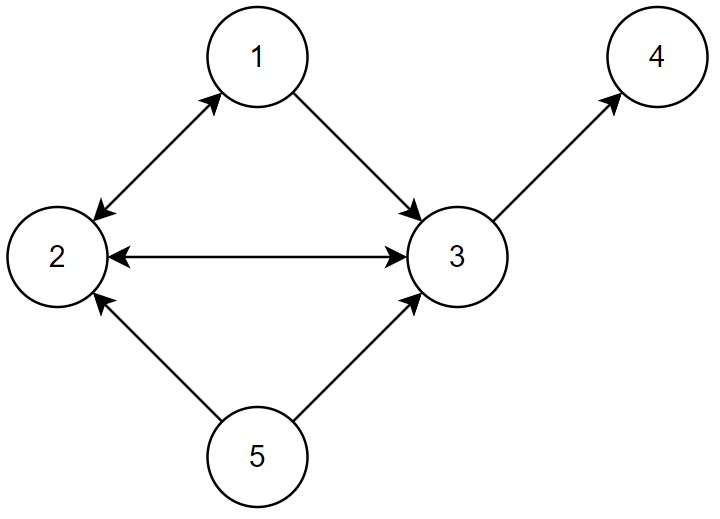
\includegraphics[width=0.5\linewidth]{images/conflictgraph2.png}
        \end{figure}
        In this case it is not possible to find a VSR schedule because it is impossible to do so without changing the final write on $s$. 
    \end{Answer}

    \newpage

    \begin{Exercise}[label=6]
        Classify the following schedule with respect to $CRT$ and $VRT$ classes: 
        \[r_5(x) r_3(y) w_3(y) r_6(t) r_5(t) w_5(z) w_4(x) r_3(z) w_1(y) \dots\]
        \[\dots r_6(y) w_6(t) w_4(z) w_1(t) w_3(x) w_1(x) r_1(z) w_2(t) w_2(z)\]
    \end{Exercise}
    \begin{Answer}[ref=6]
        Since CSR contains VSR we check with the conflict graph. To do so we first divide the schedule based on the resources: 
        \begin{itemize}
            \item $t: \: r_6 \: r_5 \: w_6 \: w_1 \: w_2$
            \item $x: \: r_5 \: w_4 \: w_3 \: w_1$
            \item $y: \: r_3 \: w_3 \: w_1 \: r_6$
            \item $z: \: w_5 \: r_3 \: w_4 \: r_1 \: w_2$
        \end{itemize}
        The nodes are $\{1,2,3,4,5,6\}$ and the arcs are found with the write-write or write-read relations found in the previous groups. So we have the following graph:
        \begin{figure}[H]
            \centering
            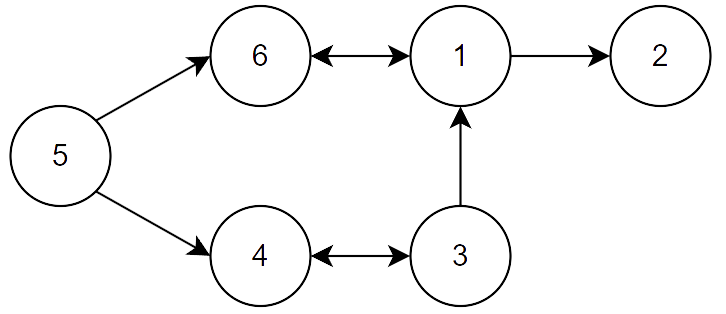
\includegraphics[width=0.5\linewidth]{images/conflictgraph3.png}
        \end{figure}
        We have two cycles. It is impossible to find a VSR schedule because only the conflict between four and three can be eliminated (the other one changes a read-write relation).
    \end{Answer}

    \newpage

    \chapter{Exercise session II}

    \begin{Exercise}[label=7]
        Classify the following schedule with respect to $2PL$ and strict $2PL$ classes: 
        \[r_1(x) r_2(y) w_3(y) r_5(x) w_5(u) w_3(s) w_2(u) w_3(x) w_1(u) r_4(y) w_5(z) r_5(z)\]
    \end{Exercise}
    \begin{Answer}[ref=7]
        For strict $2PL$ we assume that all transactions commit and release all locks immediately after their last operation, and check if releases can be executed at commit time.
        \begin{figure}[H]
            \centering
            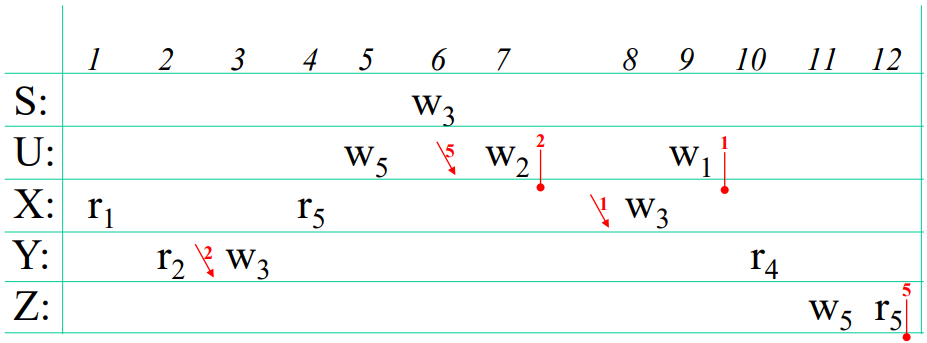
\includegraphics[width=1\linewidth]{images/2PL1.png}
        \end{figure}
        $S$ clearly cannot be in strict $2PL$. The contradictions are:
        \begin{itemize}
            \item $T_1$ must release $X$ before $8$. 
            \item $T_2$ must release $Y$ before $7$.
            \item $T_5$ must release $U$ before $12$.
        \end{itemize}
        For $2PL$ we have: 
        \begin{figure}[H]
            \centering
            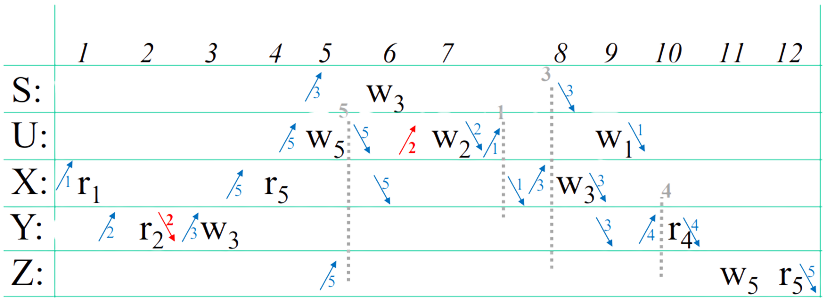
\includegraphics[width=1\linewidth]{images/2PL2.png}
        \end{figure}
        It is also not in $2PL$: an assignment is not possible for $T_2$ (which must release $Y$ before locking $U$).
    \end{Answer}

    \newpage

    \begin{Exercise}[label=8]
        Classify the following schedule with respect to $2PL$ and strict $2PL$ classes: 
        \[r_4(x) r_2(x) w_4(x) w_2(y) w_4(y) r_3(y) w_3(x) w_4(z) r_3(z) r_6(z) r_8(z) w_6(z) w_9(z) r_5(z) r_10(z)\]
    \end{Exercise}
    \begin{Answer}[ref=8]
        For strict $2PL$ we assume that all transactions commit and release all locks immediately after their last operation, and check if releases can be executed at commit time.
        \begin{figure}[H]
            \centering
            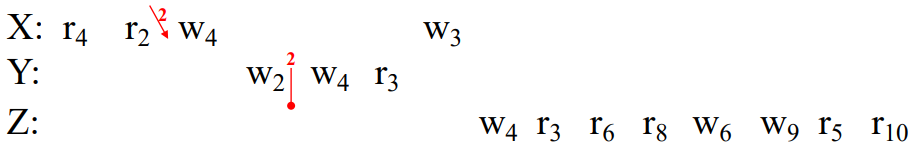
\includegraphics[width=1\linewidth]{images/2PL3.png}
        \end{figure}
        It is therefore clear that the schedule cannot be in $2PL$-strict, due to $T_2$ and $T_4$: $T_2$ ends after 4, but $T_4$ wants to write $X$ at 3, and $T_2$ would thus be 
        required to release $X$ earlier, which is impossible if $T_2$ has to keep all locks until after 4.

        For $2PL$ we have: 
        \begin{figure}[H]
            \centering
            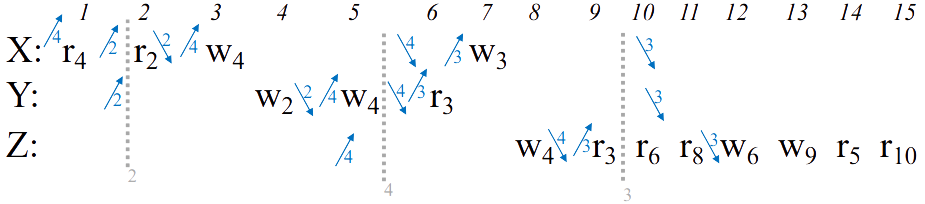
\includegraphics[width=1\linewidth]{images/2PL4.png}
        \end{figure}
        We need to look at those acquisitions that must be anticipated and to those releases that must be delayed to not violate the $2PL$ rules.
        $T_4$ can only get the XL on X only after 2 and on $Y$ after 4 and has to release $Y$ before 6 and $X$ before 7. Thus, the lock on $Z$ must be acquired before 6.
        $T_2$ can get all the locks at the beginning and release them immediately after each use. $T_3$ can acquire $X$, $Y$ and $Z$ just before using them and release them all before 12. 
        All other transactions ($T_6, T_9, T_5, T_10$) clearly pose no problems.
    \end{Answer}

    \newpage

    \begin{Exercise}[label=9]
        Classify the following schedule with respect to $2PL$ and strict $2PL$ classes: 
        \[r_1(A) r_2(A) w_2(A) r_1(B) w_1(C) w_2(C) r_3(C) w_3(A) w_2(B) w_3(B)\]
    \end{Exercise}
    \begin{Answer}[ref=9]
        For strict $2PL$ we assume that all transactions commit and release all locks immediately after their last operation, and check if releases can be executed at commit time.
        \begin{figure}[H]
            \centering
            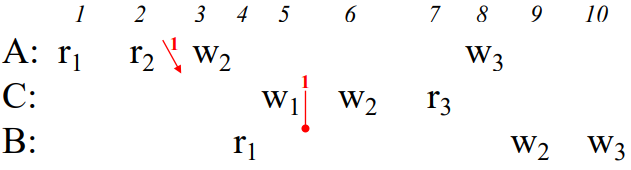
\includegraphics[width=1\linewidth]{images/2PL5.png}
        \end{figure}
        The schedule is not strict $2PL$.

        For $2PL$ we have: 
        \begin{figure}[H]
            \centering
            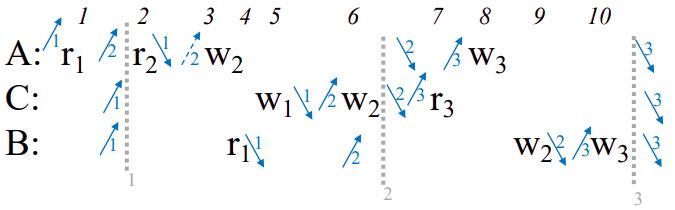
\includegraphics[width=1\linewidth]{images/2PL6.png}
        \end{figure}
        The schedule is $2PL$. 
    \end{Answer}

    \newpage

    \begin{Exercise}[label=10]
        Classify the following schedule with respect to $2PL$ and strict $2PL$ classes: 
        \[r_1(x) w_2(x) r_1(z) w_1(y) r_3(x) r_4(x) w_3(z) w_2(y) r_3(y) w_4(x) w_4(y)\]
    \end{Exercise}
    \begin{Answer}[ref=10]
        For strict $2PL$ we assume that all transactions commit and release all locks immediately after their last operation, and check if releases can be executed at commit time.
        \begin{figure}[H]
            \centering
            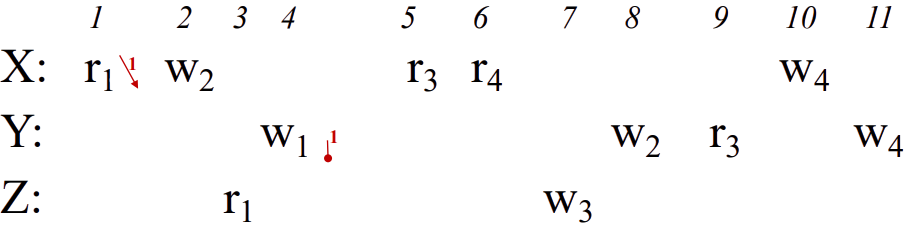
\includegraphics[width=1\linewidth]{images/2PL7.png}
        \end{figure}
        The schedule is not strict $2PL$.

        For $2PL$ we have: 
        \begin{figure}[H]
            \centering
            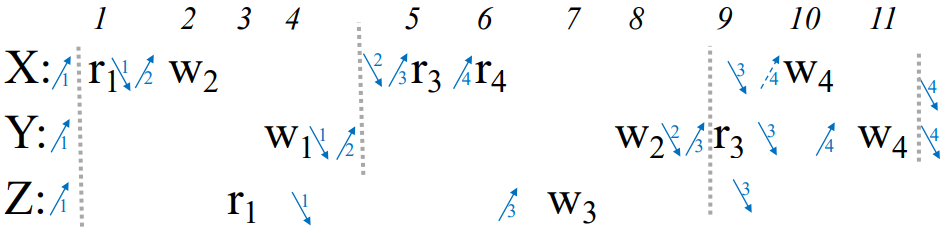
\includegraphics[width=1\linewidth]{images/2PL8.png}
        \end{figure}
        The schedule is $2PL$. 
    \end{Answer}

    \newpage

    \begin{Exercise}[label=11]
        Given the schedule:
        \[r1(x) r2(x) r3(y) w3(y) w1(x) w2(y)\]
        show the sequence of lock and unlock requests produced by the transactions in a $2PL$ execution, in a system with update lock (available locks: $SL, UL, XL$).
    \end{Exercise}
    \begin{Answer}[ref=11]
        The locking phases with update locks are the following: 
        \begin{table}[H]
            \centering
            \begin{tabular}{|c|c|}
            \hline
            $X$                                           & $Y$                                           \\ \hline
            $\textnormal{UL}_1(x)$                        &                                               \\
            $r_1(x)$                                      &                                               \\
            $\textnormal{SL}_2(x)$                        &                                               \\
            $r_2(x)$                                      &                                               \\
                                                          & $\textnormal{UL}_3(y)$                        \\
                                                          & $r_3(y)$                                      \\
                                                          & $\textnormal{XL}_3(y) [\textnormal{upgrade}]$ \\
                                                          & $w_3(y)$                                      \\
                                                          & $\textnormal{rel}(\textnormal{XL}_3(y))$      \\
                                                          & $\textnormal{XL}_2(y)$                        \\
            $\textnormal{rel}(\textnormal{SL}_2(x))$      &                                               \\
            $\textnormal{XL}_1(x) [\textnormal{upgrade}]$ &                                               \\
            $w_1(x)$                                      &                                               \\
            $\textnormal{rel}(\textnormal{XL}_1(x))$      &                                               \\
                                                          & $w_2(y)$                                      \\
                                                          & $\textnormal{rel}(\textnormal{XL}_2(y))$      \\ \hline
            \end{tabular}
        \end{table}
    \end{Answer}

    \newpage

    \begin{Exercise}[label=12]
        Update lock was introduced to contrast deadlocks. Can we state that deadlocks are impossible in the presence of update locks?
        \begin{enumerate}
            \item If so, concisely explain why. 
            \item If not, provide a counter-example.
        \end{enumerate}
    \end{Exercise}
    \begin{Answer}[ref=12]
        \begin{enumerate}
            \item Clearly deadlocks are possible in the presence of UL. Indeed, UL only makes deadlock less likely, by preventing one type of (very frequent) deadlock, due to 
                update patterns, when two transactions compete for the same resource ($r_1(x) r_2(x) w_1(x) w_2(x)$). 
            \item Consider two distinct resources $X$ and $Y$, and two transactions that want to access them in this order: $r_1(X) r_2(Y) w_1(Y) w_2(X)$. It is likely that they end up 
                in deadlock, especially if the system on which they run applies $2PL$. UL is totally irrelevant here, because there is no update pattern. 
        \end{enumerate}
    \end{Answer}
\end{document}